\chapter{Evaluation of the ICE--Model}\label{modelanalysis}
We now have a complete geomtrical representation of the ICE model as well as
 the analytical expressions $u_0$ and $u_L$ that describe the membrane displacements
in spatial detail as a function of direction and frequency. In this chapter we will use these variables
to further study the features and predictions of our model and compare them with experimental results. In
order to completely explain the obeservations, we will also need to estimate certain physical parameters
like membrane eigenfrequency and quality factor that are important to our analysis but haven't yet been
experimentally measured.

The main body of this chapter proceeds in Sec. \ref{localizationsection} directly from the definitions given in \eqref{ipsimembranefull}
and \eqref{contramembranefull}. We will begin by assigning numerical values to the model parameters that have been defined
in the previous chapter and comparing the membrane velocities of our model with experimentally determined values. 
We will then go on to define define and study the two main quantities that serve as important localization
cues - the Internal Time Differences (iTDs) and the Internal Level Differences (iLDs). 
These values model the 
possible neural subtractions that take place in the animal's brain in order to enhance directional sensitivity. Upon obtaining 
the spectral behaviour of these quantities, we will also be able to make an educated guess about
the respective frequency ranges in which these cues are dominant and the possible range in which they could simultaneously
be used. 
We will end this section
by discussing the methods we have used to estimate the parameter values.
% A complete evaluation of our model also requires  a discussion of the 
% pressure distribution profile and eigenfrequencies of the mouth cavity which will be done in Sec. \ref{pressuredistchapter}.
Finally, in Sec \ref{vibrationpatternchapter} we will compare the experimentally determined vibration pattern
of the Tokay gecko's eardrum with that of our model's eardrum - the aim being to justify our choice for the
geometry of the membrane.

In order to underline the fact that our model is universal model for internally coupled ears and not
specialized to single species, we will compare our results for two gecko species - \textit{Hemidactylus frenatus}
or the common house gecko and the Tokay gecko. At the end of the chapter we will have an understanding of the advantages of a coupled system of ears as opposed
to a pair of independent ears. We will also have an idea about the frequency regimes that correspond to the use
of iTDs and iLDs in localization.


\section{Sound Localization Using the ICE Model}\label{localizationsection}
In our study we are primarily concerned with hearing in geckos. We will be using
parameters (interaural separation, tympanum area etc.) from \textit{Hemidactylus frenatus}, the common house gecko
\cite{dalsgaardmanley2} and the Tokay gecko \cite{dalsgaardmanley1}, \cite{dalsgaardtangcarr}. In order to proceed
with our evaluation of our model, we will need to assign appropriate numerical values to the parameters we have
defined in \ref{parametertable}. For now we will simply list the values and leave the discussion to a later point.

\vspace{\baselineskip}
\noindent
\begin{minipage}{\linewidth}
\renewcommand{\arraystretch}{1.3}
%\caption{Parameters and Functions used in the ICE Model} \label{parametertable} 
\centering
\captionof{table}{ICE Model geometry Parameters for the common house gecko (Hemidactylus frenatus) and the Tokay gecko.}\label{geckogeometricparams}
\begin{tabular}{|p{8.5 cm} | c | c|}
\hline
Parameter name & Hemidactylus & Tokay gecko\\
\hline
Length of the cylinder or interaural distance, L & $10$mm & $22$mm\\
Radius of the tympanic membrane, $a_{tymp}$& $1.5$mm & $2.6$mm\\
Fundamental frequency (first eigenfrequency) of the tympanic membrane, $\omega_{01}$ & $3200$Hz & $1050$Hz\\
Quality factor of the tympanum, $Q$ & $1.3$ &  $1.4$\\
Density of the membrane material, $\rho_m$ & $1$mg/mm$^3$ & $1$mg/mm$^3$\\
Thickness of the membrane, $d$& $8\mu$m & $10\mu$m\\
Volume of the cavity, $V_{cav}$ & $.32$ml & $3.5$ml\\ 
Extracolumella angle, $\beta$ & $\pi/25$ & $\pi/25$\\
Cylinder radius calculated from $V_{cav}$ and $L$ using the formula given in \eqref{cylinderradiusformula}, $a_{cyl}$ & $\sim 6.6$mm  &$\sim 3.2$mm \\
\hline
\end {tabular}\par
\bigskip
\end{minipage}
From these quantities it should be apparent that the house gecko, with an interaural separation of $10$mm and mouth cavity volume of $.32$ml is a rather
small lizard. The Tokay gecko is the second largest gecko species (interaural separation of $22$mm and mouth cavity volume $3.5$ml, \cite{dalsgaardmanley2}).
Thus we will demonstrate the scalability of our model with regards to hearing in animals with widely varying head widths and mouth cavities. As we will subsequently see, the geometric parameters, especially
the head width and the membrane eigenfrequencies, put important limits on the ``hearing range'' of our model.

Before we begin our comparison of the data, we should first acquaint ourselves with some experimental details. As already mentioned in Sec. \ref{soundinput}, the geckos were placed in
an anechoic room. They were subject to $175$ms frequency sweeps (200-7500 Hz) at levels of 80-90 dB with the speakers placed at
a $1$m distance. The eardrum vibrations were then measured using laser-Doppler vibrometry with the point
of measurement at the tip of the extracolumella. The measured values correspond to the displacement velocity of the membrane at this point.  
In our analysis, the point corresponding to the tip of the extracolumella is stationary and cannot be used to compare the vibrations of the membranes. 
Instead, we use the total membrane displacements defined in the previous chapter which are given by,
\begin{align}
 &S^0=G^s_{ipsi}p_0+G^s_{contra} p_L\\
 &S^L=G^s_{ipsi}p_L+G^s_{contra}p_0\\
 &\dot{S}^{0/L}=j\omega S^{0/L}\label{totalvelocity}
\end{align}
using the ipsi- and contralateral filters for the total displacement defined in \eqref{ipsimembranetotal} and \eqref{contramembranetotal}.
The definition of the total membrane velocity given in the second line follows directly from the definition of the membrane displacements. Following Sec. \ref{soundinput}
and \eqref{oldsoundinput}, the sound pressure inputs have the form
\begin{equation}\label{newsoundinput}
 p_0=pe^{j\omega t} e^{j\Delta_{new}/2},\qquad p_L=pe^{j\omega t} e^{-j\Delta_{new}/2},\qquad \Delta_{new}=1.5kL\sin\theta.
\end{equation}
The rest of this section follows from the above definitions. In Sec. \ref{vibvelocity} we study the dependence of the membrane vibration velocity 
on the frequency and direction of the sound source. Using the membrane vibration velocity we will define the main directional hearing cues
 - the Internal Time and Level Differences - in Sec. \ref{hearingcuessection}. As mentioned earlier, we will conclude by justifying our selection of parameters. In
Sec. \ref{parameterestimation} we will analyse the dependence of the expressions defined in previous sections on the system parameters 
and in this way also provide estimates for realistic material parameters.
\subsection{Membrane Vibration Velocity}\label{vibvelocity}
In this section we will see how the total membrane displacements accurately
represent the response of the membrane to external stimuli. Before we begin, we should note that although the quantities
$\dot{S}^{0/L}$ will not quantitatively reproduce the experimentally measure membrane vibrations, their behaviour with respect to
frequency and direction is consistent. They also have the added advantage that they only depend on direction and frequency. In Fig. \ref{hemidactylusvibampfull},
we compare the normalized velocity of the tympanic membrane ($\dot{S}^{0/L}/(\pi a^2_{cyl})$) with the membrane velocity measured using laser vibrometry
in \cite{dalsgaardmanley2}. The plot shows the vibration amplitude as a function of frequency ($y$-axis) and direction ($x$-axis). The amplitudes are given
is units of dB re $1$ mm/(s Pa). This means that we have plotted the ratio vibration amplitude with reference to a vibration velocity of $1$ mm/s with an input pressure of $1$ Pa.
In other words we have set $p=1$Pa in \eqref{newsoundinput}.
\begin{figure}[ht!]
 \centering
 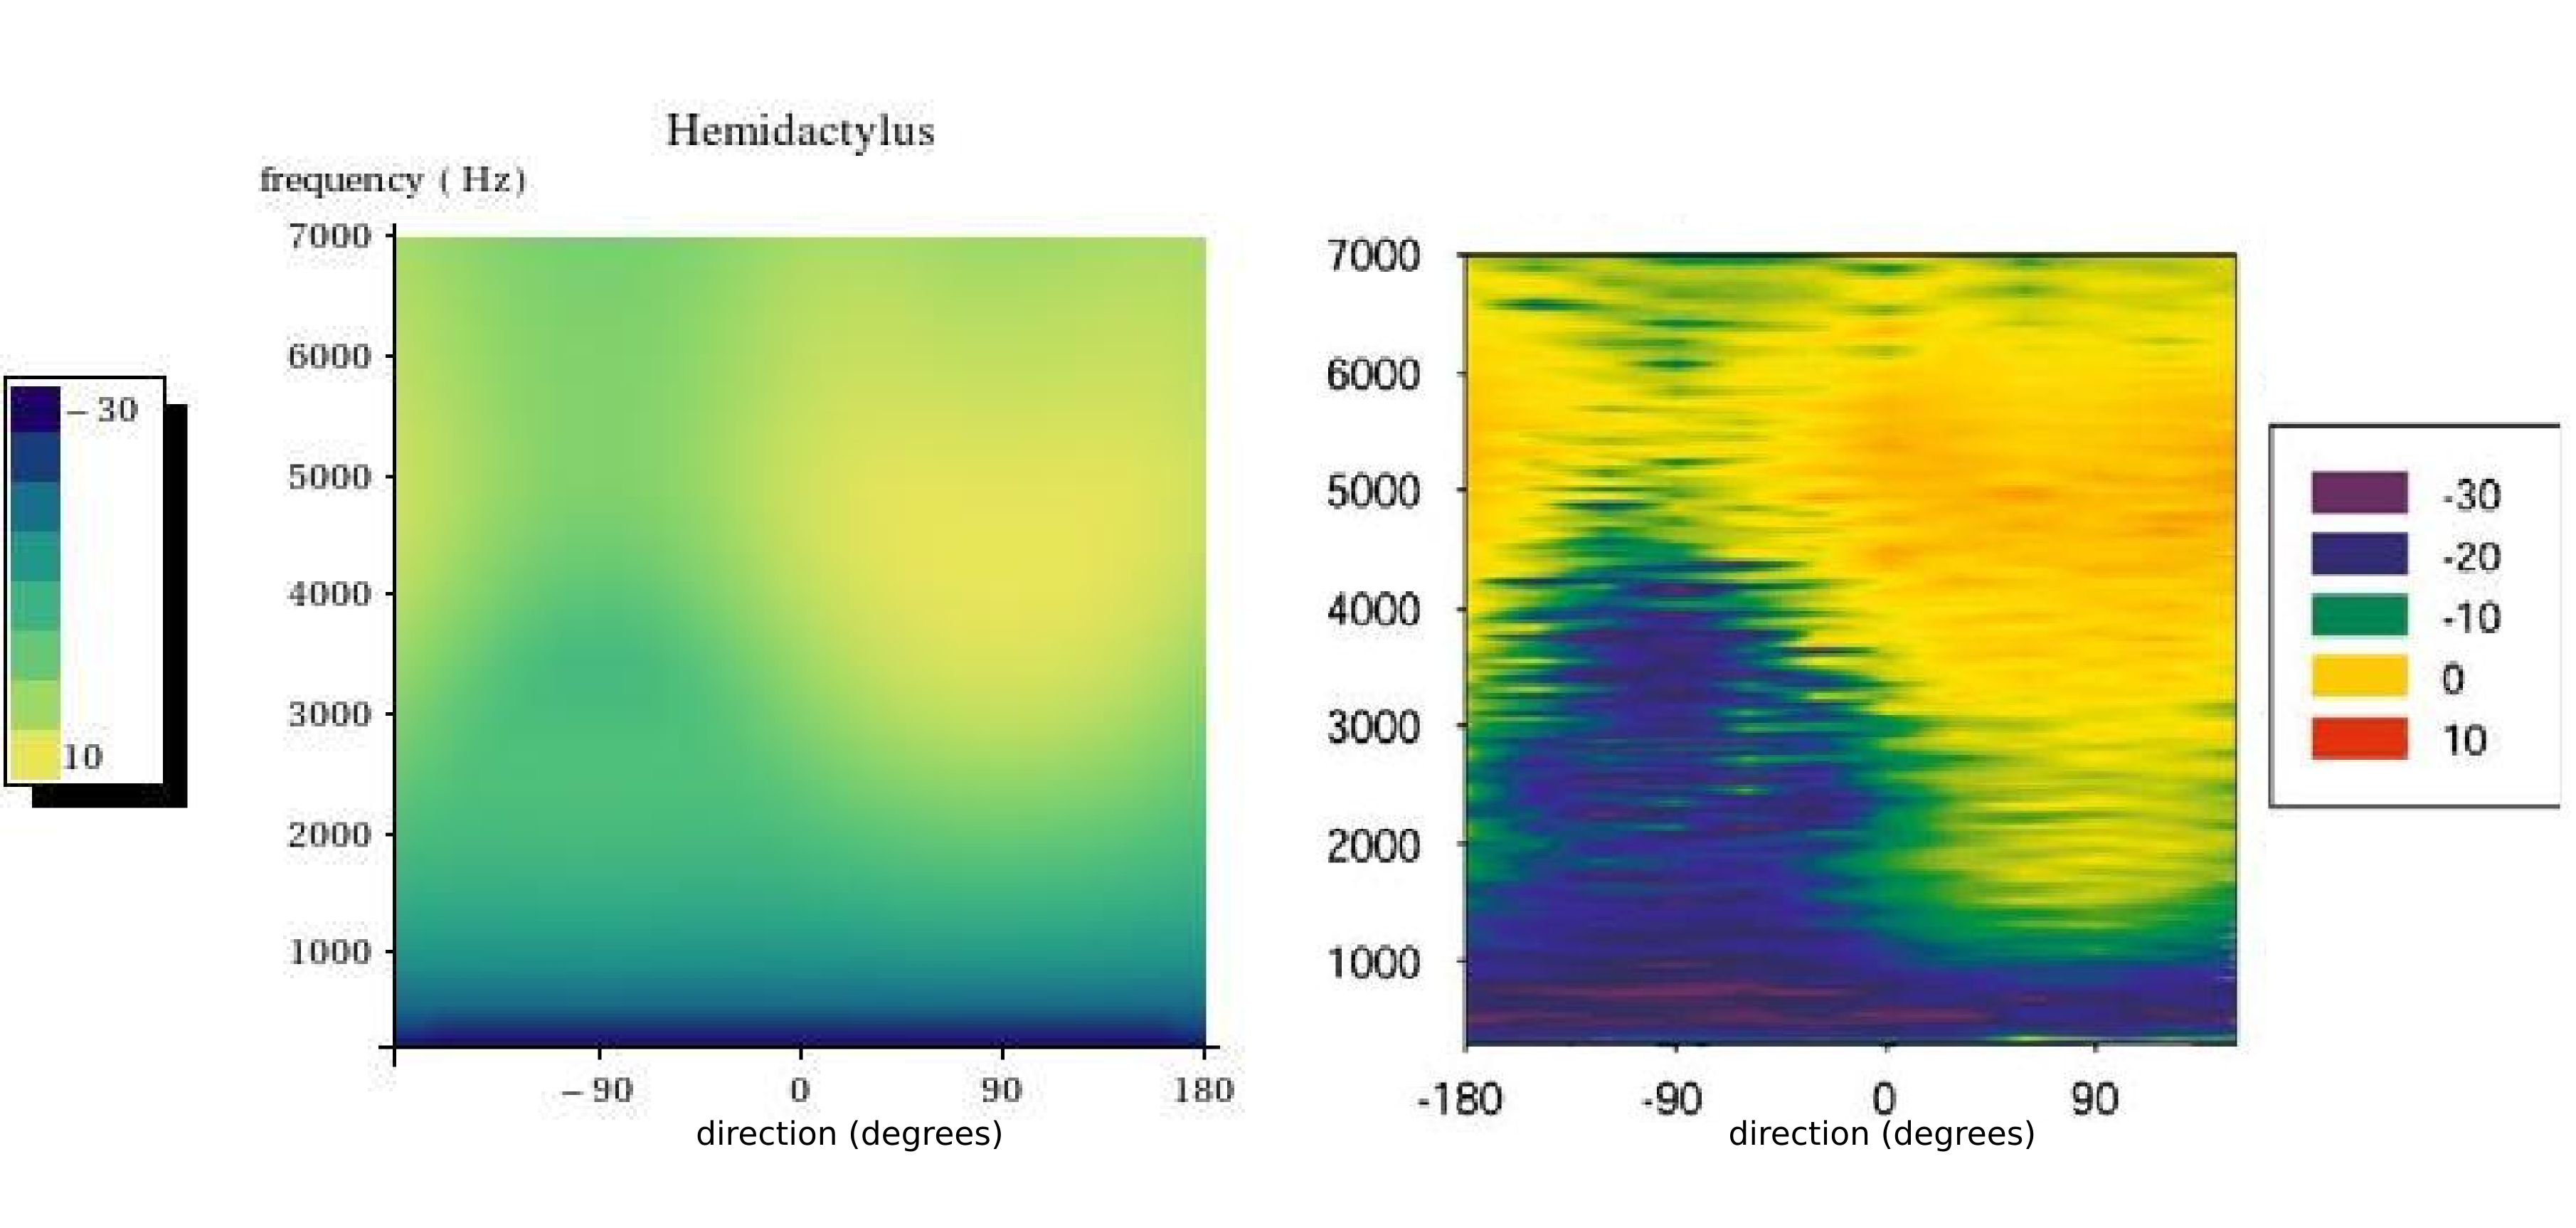
\includegraphics[width=1.0\linewidth]{Diagrams/Plots/hemidactylusvibampfull.png}
 \caption[Vibration amplitude for the common house gecko]{Calculated (left) and experimental (right) amplitude of tympanic membrane vibrations for Hemidactylus frenatus
 in dB re $1$ mm/(s Pa), i.e. the ratio of the vibration amplitude with reference to a vibration velocity of $1$ mm/s with an input pressure of $1$ Pa. On the $x$-axis we have
 the direction of the sound source in degrees varying from $-180^\circ\mbox{ to }180^\circ$ with positive angles corresponding to ipsilateral stimuli. The legends on the left and
 right denote the amplitude in decibels. The calculate values are from the ICE model and the experimental values are taken from Christensen-Dalsgaard \cite{dalsgaardmanley2}.}
  \label{hemidactylusvibampfull}
\end{figure}

As we can see, the total membrane velocities reproduce the frequency and direction dependence of the system fairly well. The directional behaviour is consistent with regard
to the requirement that the membrane have a higher vibration amplitude when it is on the same side as the object. The reason for the deviation from experimental behaviour at 
higher frequencies isn't currently known. The mechanics of the extracolumella including its flection and the influence of the realistic shape of the mouth cavity could offer possible explanations.
Although the room was tested to be anechoic to below $200$Hz some reflections, especially from
the laser setup are unavoidable. This is the cause of the spectral ripple in the experimental measurements. The same comparison is illustrated for the Tokay gecko in Fig. \ref{tokayvibampfull} (data from \cite{dalsgaardmanley1}).
\begin{figure}[ht!]
 \centering
 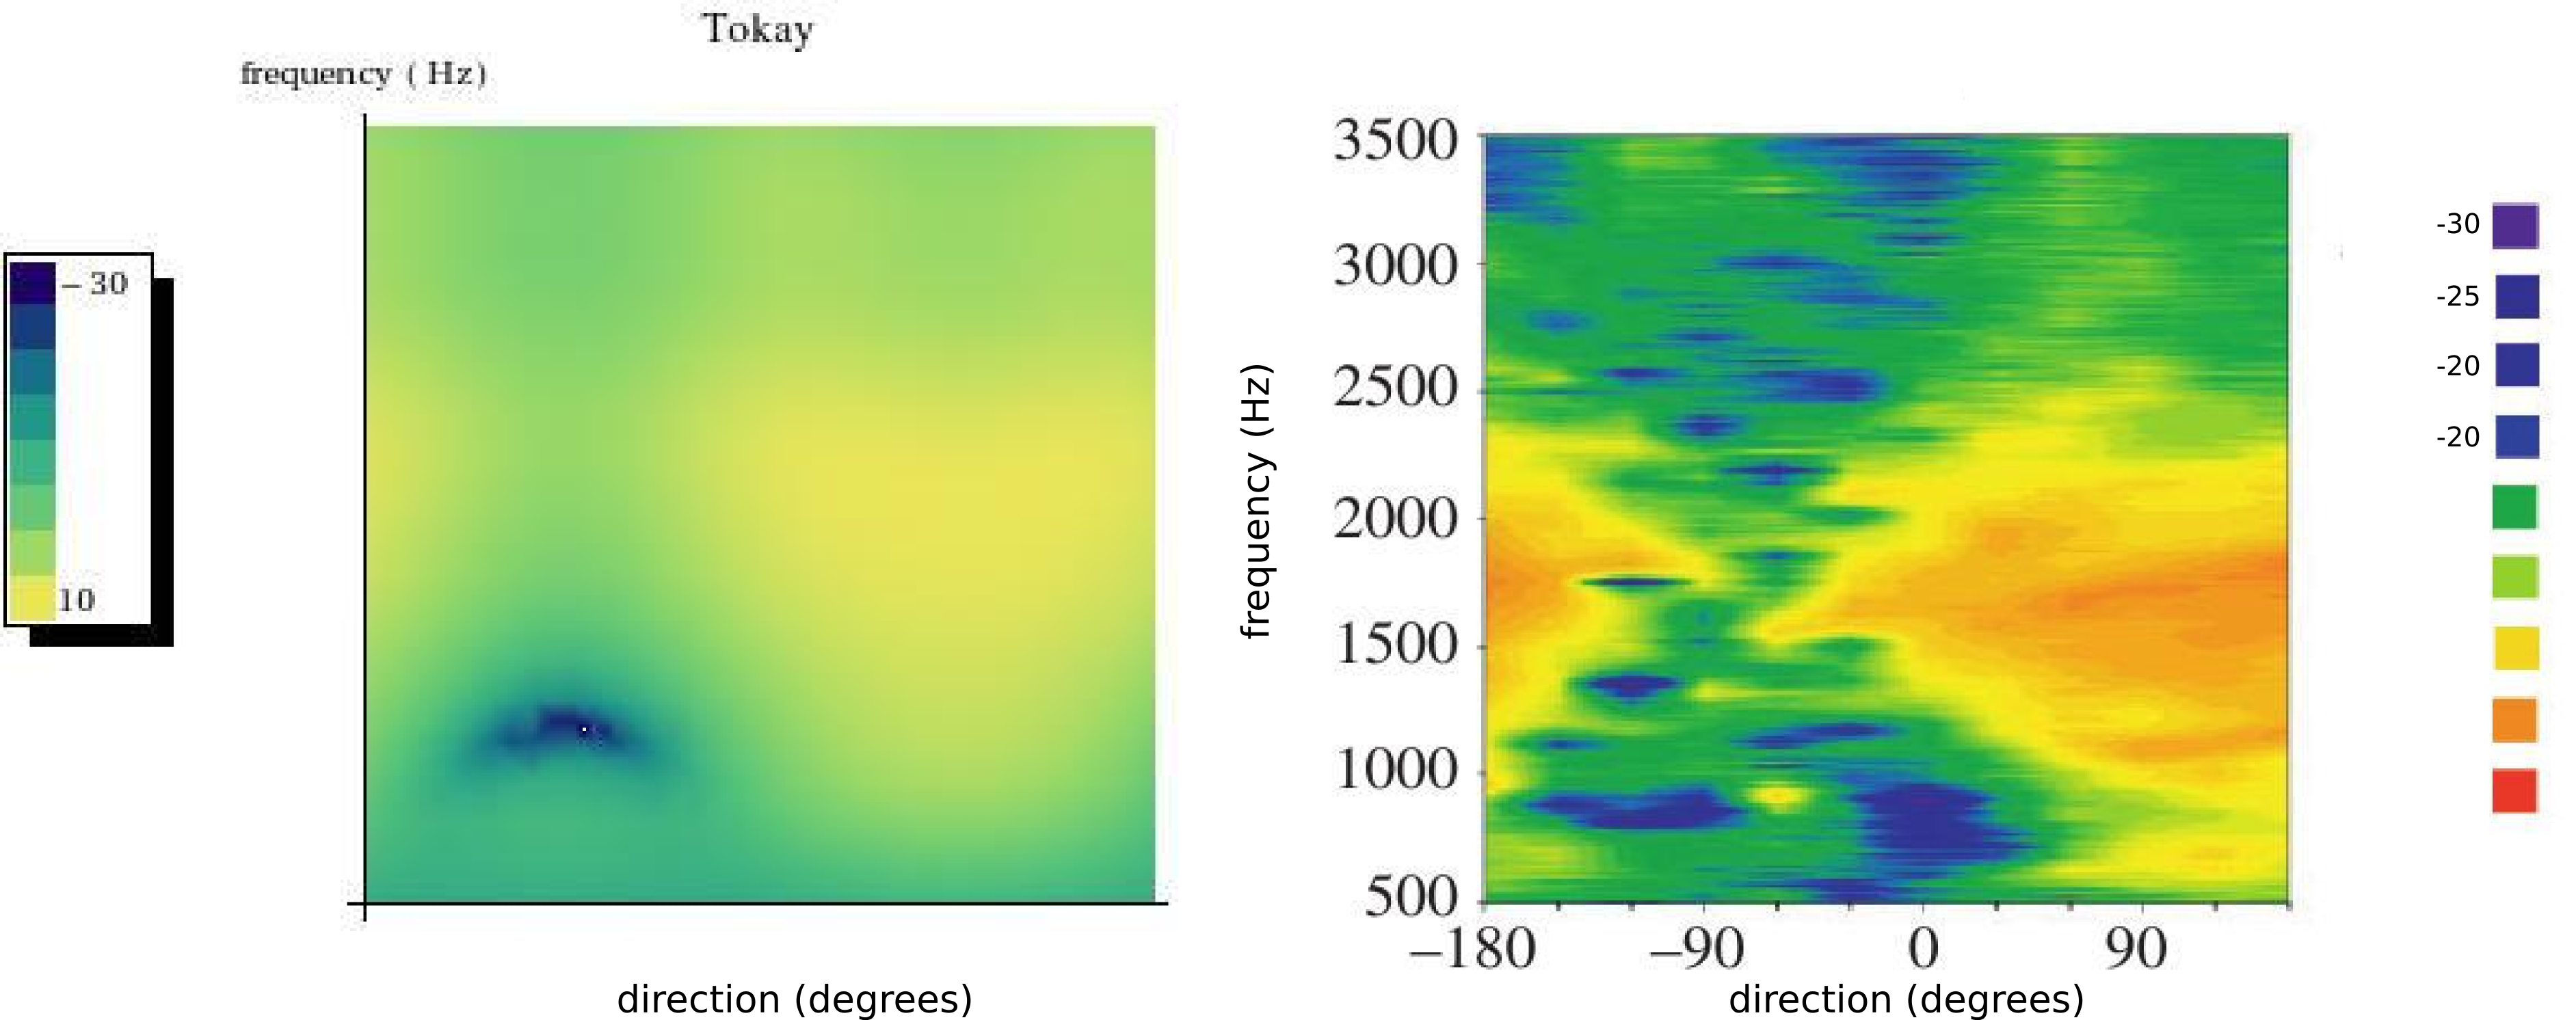
\includegraphics[width=1.0\linewidth]{Diagrams/Plots/tokayvibampfull.png}
 \caption[Vibration amplitude for the Tokay gecko]{Calculated (left) and experimental (right) amplitude of tympanic membrane vibrations for the Tokay gecko
 in dB re $1$ mm/(s Pa). The axis and legend values are the same as the ones in Fig. \ref{hemidactylusvibampfull}. The experimental values are taken from Christensen-Dalsgaard \cite{dalsgaardmanley1}.}
  \label{tokayvibampfull}
\end{figure}

In order to get a better understanding of the directionality of the model, it is also important to look at the dependence of the vibration amplitudes on direction and frequency independently. 
In Fig. \ref{hemidactylusipsivscontrafull} (house gecko)
and Fig. \ref{tokayipsivscontrafull} (Tokay gecko) we have plotted the membrane vibration velocity for a pure ipsilateral stimulus (90$^\circ$) and pure contralateral stimulus (-90$^\circ$)
as a function of frequency.
\begin{figure}[ht!]
 \centering
 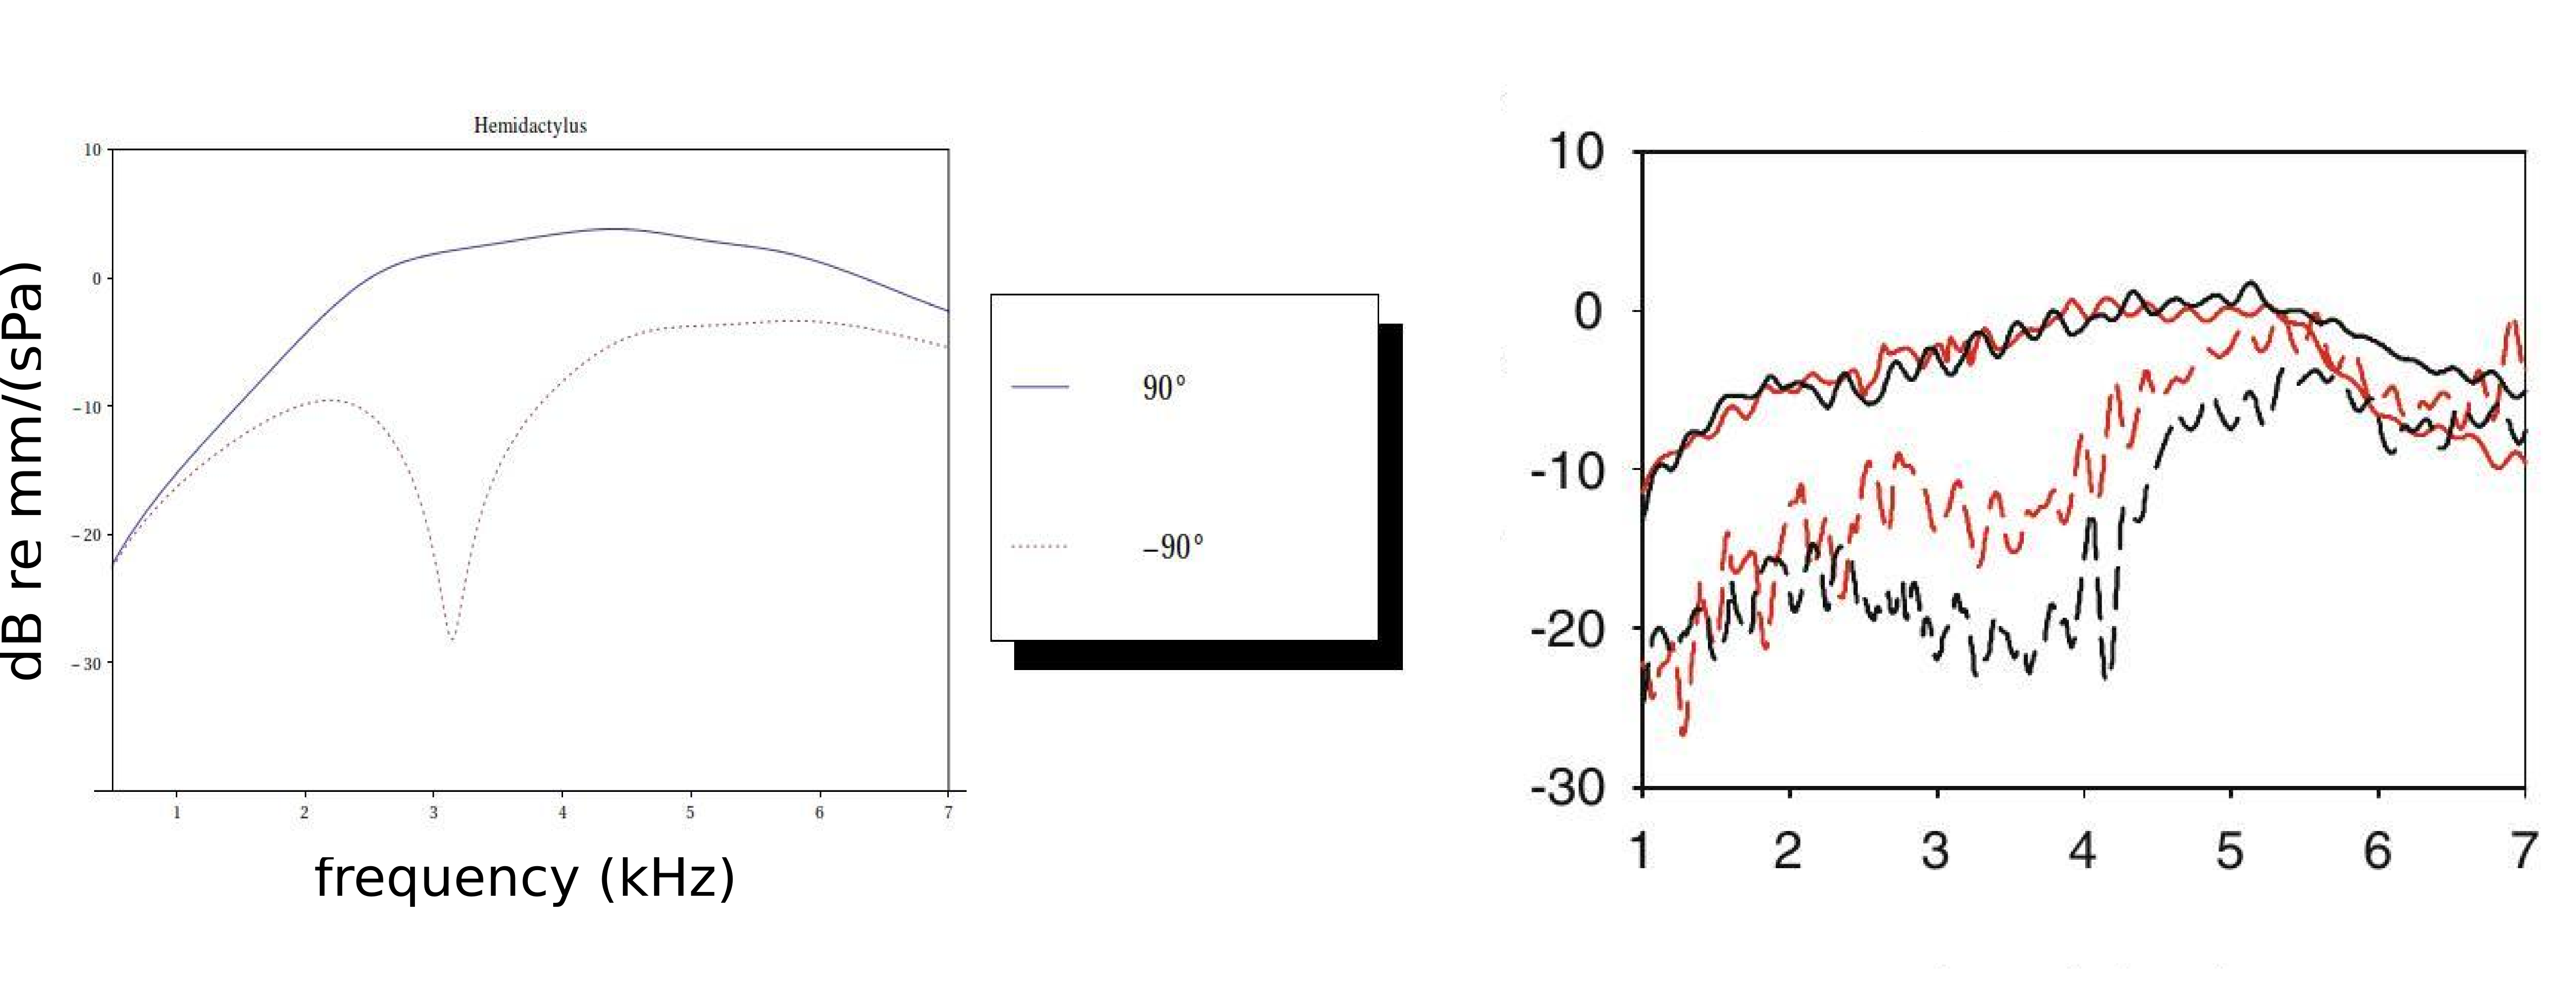
\includegraphics[width=1.0\linewidth]{Diagrams/Plots/hemidactylusipsivscontrafull.png}
 \caption[Frequency dependence of ipsi- and contralateral membrane vibration amplitudes - common house gecko]{Calculated (left) and experimental (right) vibration velocity spectra for the common house gecko. The two plots
 on the left correspond to the response of the tympanic membrane to a purely ipsilateral (90$^\circ$) and purely contralateral (-90$^\circ$) stimulus.  The two colours on the right correspond to
 different individuals of the house gecko species. Experimental values taken from Christensen-Dalsgaard \cite{dalsgaardmanley2}.}
  \label{hemidactylusipsivscontrafull}
\end{figure}
As we can see the ipsilateral response is generally higher than the contralateral response and the difference peaks at a certain frequency i.e., it
has a bandpass characteristic which is consistent with observations.
These amplitude differences can be used to localize the sound source; see Sec. \ref{hearingcuessection}. At very low and very high frequencies the both the vibration amplitudes
converge.  In Fig. \ref{freqdepboth} we  have also plotted the response of the ear to ipsi- and contralateral stimuli with varying directions. (90$^\circ$,60$^\circ$,0$^\circ$,-60$^\circ$,-90$^\circ$)
and thereby shown that the vibration amplitude is higher when the sound source is nearer to the ear (i.e. $\theta$ is closer to $90^\circ$).
\begin{figure}[ht!]
 \centering
 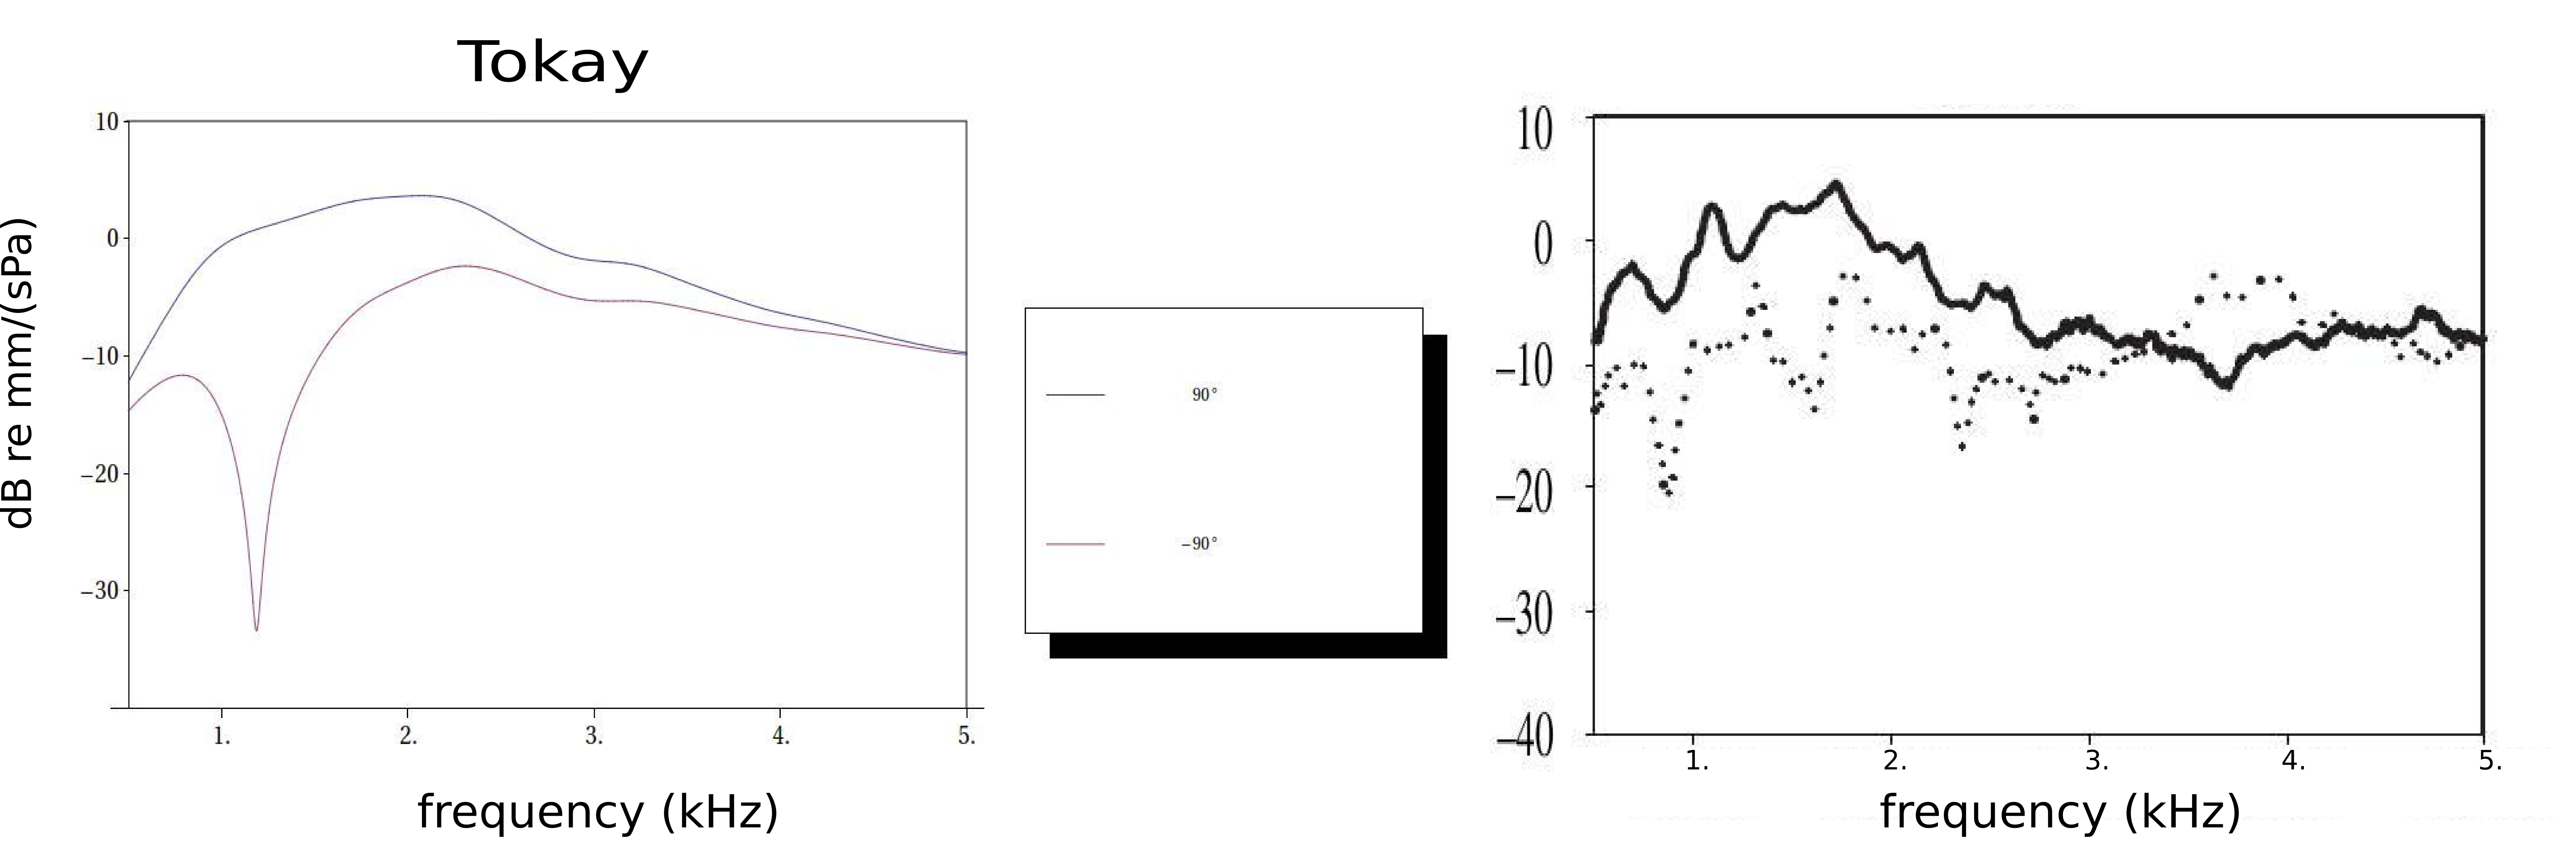
\includegraphics[width=1.0\linewidth]{Diagrams/Plots/tokayipsivscontrafull.png}
 \caption[Frequency dependence of ipsi- and contralateral membrane vibration amplitudes - Tokay gecko]{Calculated (left) and experimental (right) vibration velocity spectra for the Tokay gecko. In
 the plot on the right hand side, the thick line corresponds to an ipsilateral stimulus and the dotted line to a contralateral stimulus.  Data from \cite{dalsgaardmanley1}.}
  \label{tokayipsivscontrafull}
\end{figure}
\begin{figure}[ht!]
\centering
  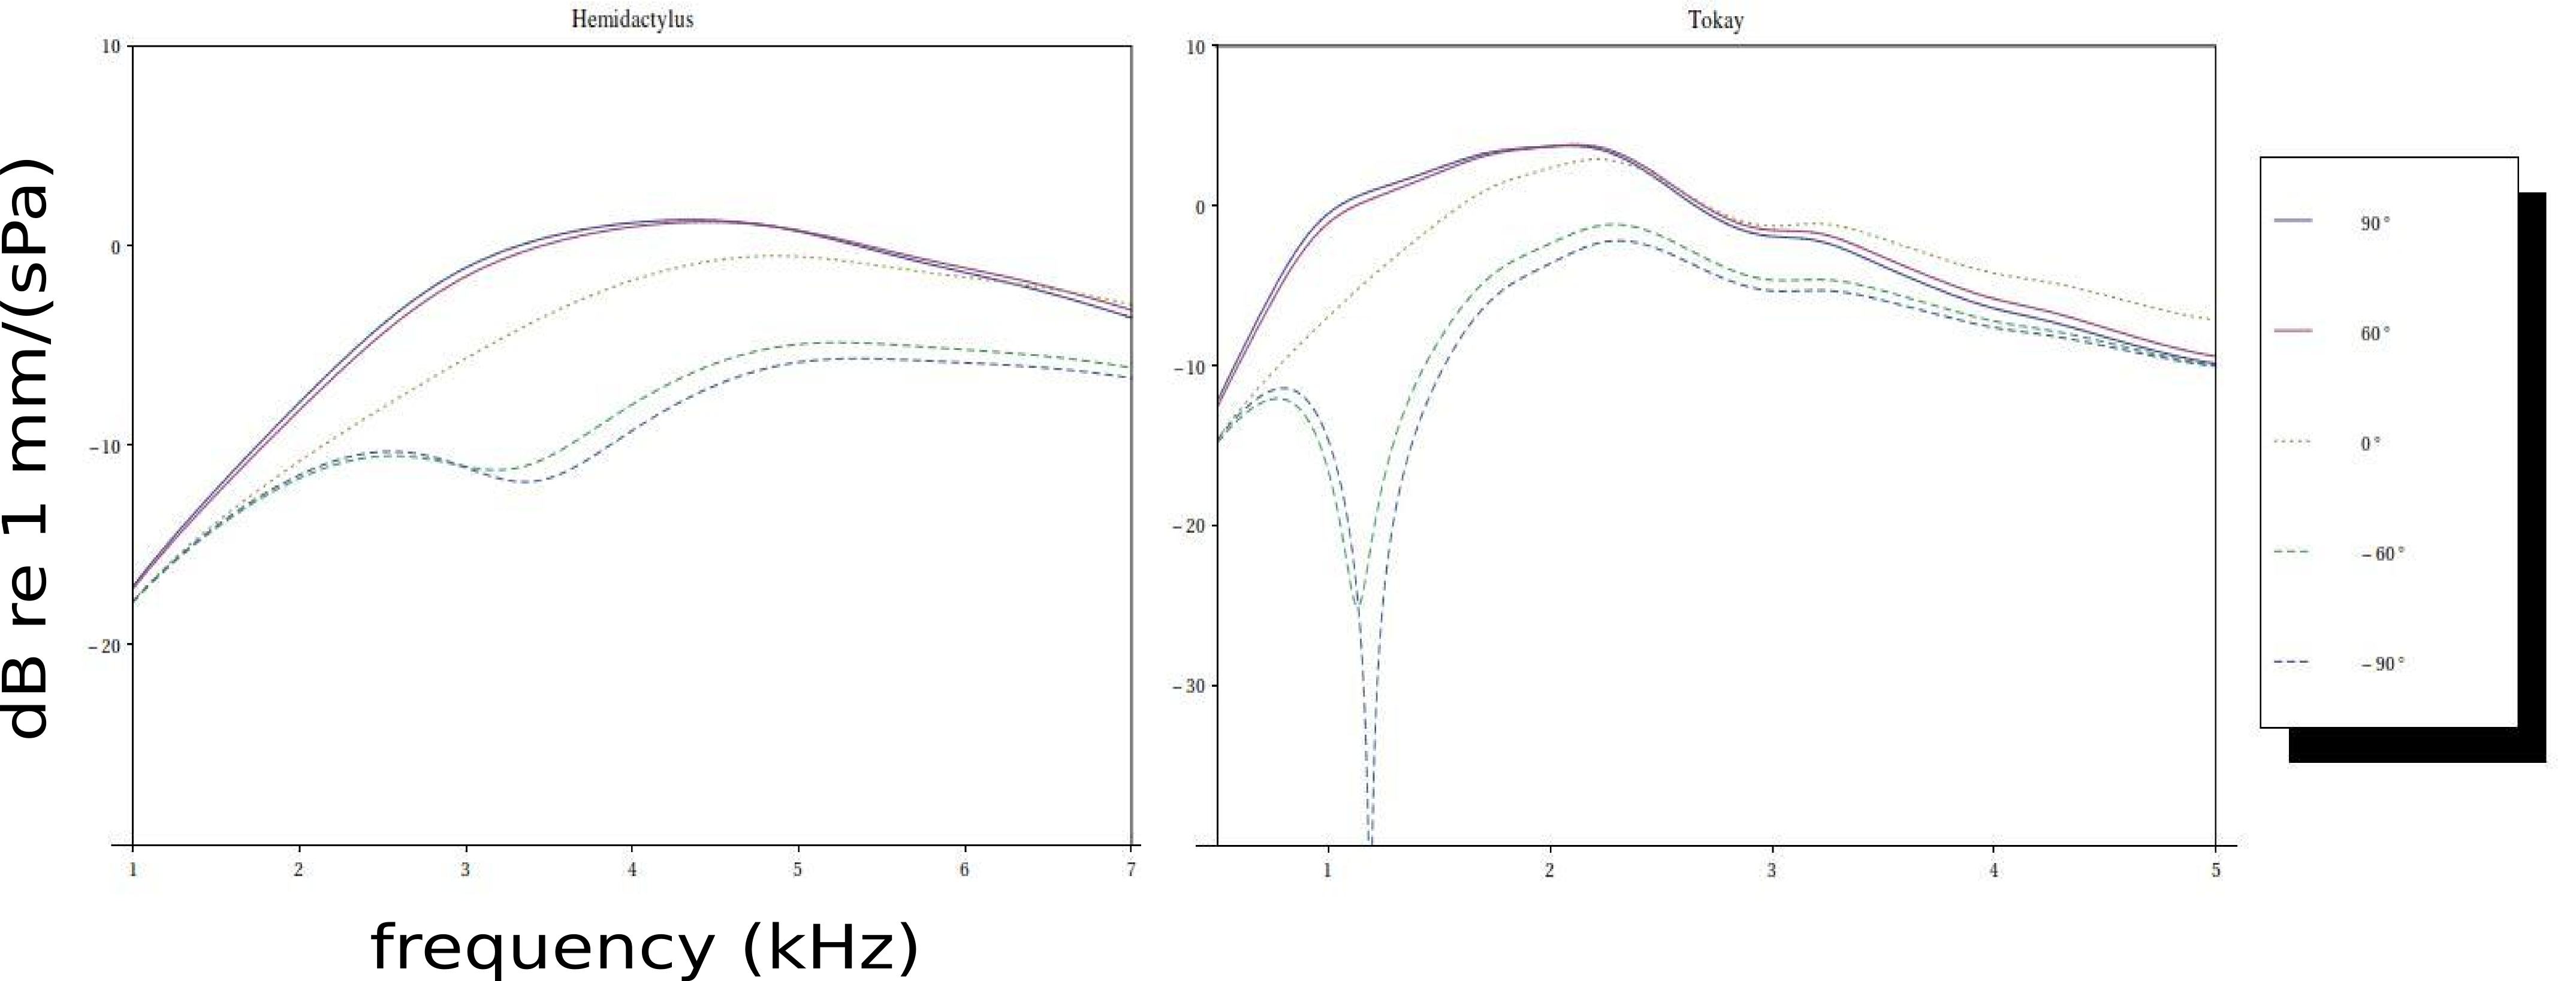
\includegraphics[width=1.0\linewidth]{Diagrams/Plots/freqdepboth.png}
  \caption[Frequency dependence of membrane vibration amplitudes for different directions.]{Frequency dependence of membrane vibration amplitudes for different directions - common house gecko (left), Tokay gecko (right). 
  The amplitude response to ipsilateral stimuli is generally higher and is at a maximum when the object is nearest to the ear i.e. $\theta=90^\circ$. The dotted line denotes a sound source directly in front of or behind the animal and the dashed lines denote contralateral stimuli.}
  \label{freqdepboth}
\end{figure}

We conclude this section by looking at the directional dependence of the vibration for a given set of frequencies. In Fig. \ref{directionplots}, we show the variation of the vibration amplitude of the membrane as
the sound source moves around the animal i.e. as $\theta$ varies from $-180^\circ$ to $180^\circ$.
\begin{figure}[ht!]
\centering
  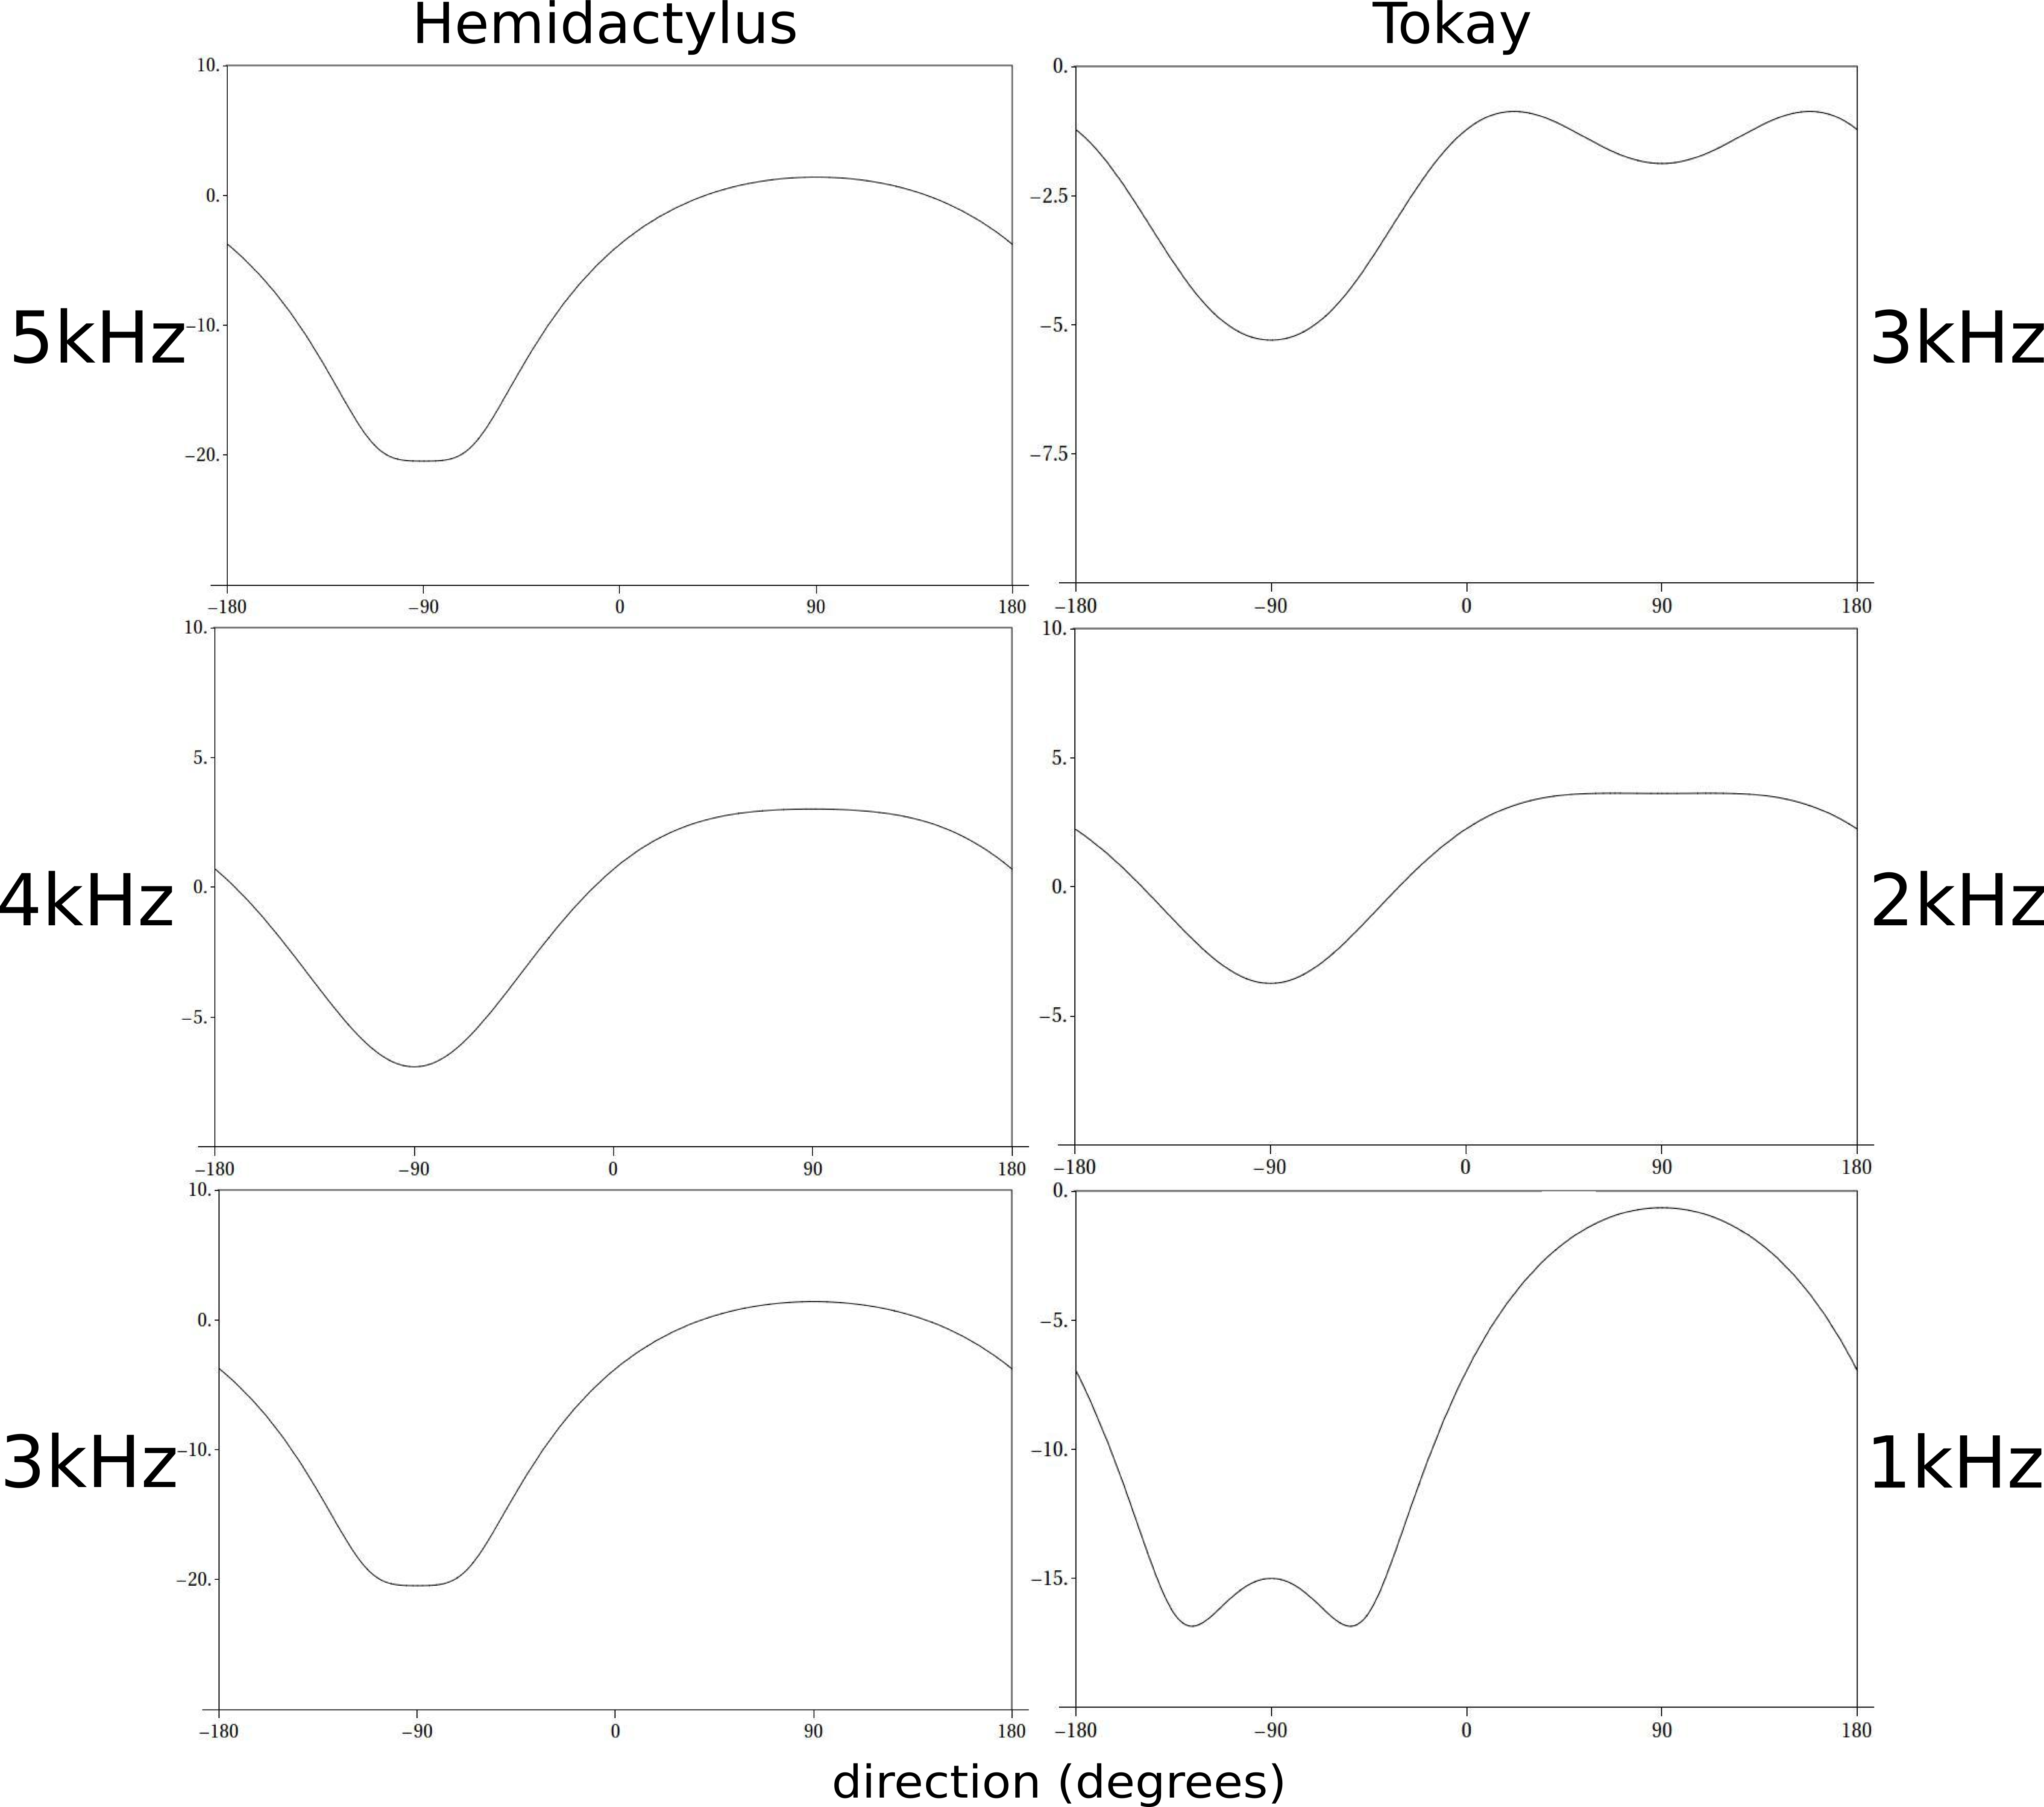
\includegraphics[width=.5\linewidth]{Diagrams/Plots/directionplots/directionplots.png}
  \caption[Direction dependence of membrane vibration amplitudes for different frequencies.]{Direction dependence of membrane vibration amplitudes  in the ICE Model for different frequencies - common house gecko (left, at 3kHz, 4kHz and 5kHz)
  , Tokay gecko (right, at 1kHz, 2kHz and 3kHz).
  The variation of the amplitude as the sound source completes a full circle around the animal is illustrated. The amplitudes for ipsilateral stimuli are shown to be
  higher than those for contraletaral stimuli.}
  \label{directionplots}
\end{figure}
Here we can more clearly see that the amplitudes due to ipsilateral stimuli are higher than those due to contralateral stimuli. The marked asymettry and the steepness across the midline (i.e. at $0^\circ$)
is also consistent with observations (\cite{dalsgaardmanley1}, \cite{dalsgaardmanley2}). The choice of our frequencies has to do with the typical hearing ranges of the geckos. The smaller house
gecko is most sensitive at higher frequencies (~3kHz) and the larger Tokay gecko at lower frequencies (~1kHz).

\subsection{Directional Hearing Cues}\label{hearingcuessection}
The significance of our results upto this point should
already be apparent. Due to the relatively small head sizes of the geckos, the sound arriving at the two ears differ very slightly in phase and not at all in amplitude. On the other hand
 these animals overcome the problem and create direction dependent differences between the vibration amplitudes of the membranes through the use of coupled ears. From
 form of the direction dependence of the membrane vibration amplitudes we see that individual amplitudes don't necessarily vary much with direction. In other words, although
 there is a clear difference between the ipsilateral and contralateral response, the difference between a given pair of ipsi- or contralateral directions (eg. between $90^\circ$
 and $75^\circ$ or between $-90^\circ$ and $-70^\circ$) isn't very significant. Therefore,
 in order to localize an object by using the tympanic membrane vibration amplitudes, we need to compare the variation of their differences with respect to direction.
 
Now that we have the vibration amplitudes of the tympanic membranes as a function of direction and frequency,
we need functions that quantify the directional dependence of the system. 
%\newcommand{\defeq}{\vcentcolon=}
As a first step we define the two quantities that are the main focus of this chapter - the internal level difference (iLD) and internal time difference (iTD)
in terms of the total membrane velocities. 
\begin{align}
  \mbox{iLD}&\vcentcolon= 20\mbox{Log}_{10}\left(\left|\frac{\dot{S}^0}{\dot{S}^L}\right|\right)\\
  \mbox{iTD}&\vcentcolon= \mbox{Arg}\left(\frac{\dot{S}^0}{\dot{S}^L}\right)/\omega.
\end{align}
Due to the steady state approximation we have the added advantage that the ratio of the displacement amplitudes is equal
to that of the velocity amplitudes; see \eqref{membraness1}. The main advantage of the velocity amplitudes 
is their relative ease of measurement in experiments. The iLD measures the ratio between the amplitudes of the eardrums and is the same as the IVAD function defined by J\o{}rgensen et al. \cite{jorgensenschmitz} and
is measured in dB. The iLD is positive for ipsilateral directions and negative for contralateral.
This agrees with observed behaviour and means that the response of the system is directional.  The iTD corresponds to the time
difference (or equivalently phase difference) between the membrane vibrations. The ipsilateral ear is always ahead in phase
with respect to the contralateral ear. This means that it is negative for ipsilateral directions and positive for contralateral.

The iTD and iLD can be seen as the output of the ICE system with $p_0$ and $p_L$ as inputs.
In contrast, the Interaural Time and Level Differences (ITD and ILD) are entirely determined 
by the inputs to the two ears. The ITD is defined as the time sound takes to travel across
the head width and is given by ITD$=L/c$. It is equivalent to $\Delta$, the phase difference
between the vibrations of the eardrums without coupling and diffraction effects; see \eqref{oldsoundinput}. Due to the 
input pressures having the same amplitude and due to the linearity of the system (w.r.t sound input), the ICE model does not have any 
a priori Interaural Level Difference. In larger animals
like humans the difference between the input amplitudes increases with frequency due to 
diffraction effects (shadowing) which aids in localization; cf. \cite[p~.154]{fletcheracoustic}. In addition, the gain in ITD due
to their increased head size also provides sufficient information for localization at lower frequencies.

In order to effectively function as cues for localization the iLDs and iTDs should ideally satisfy the following requirements,
\begin{itemize}
 \item They should increase with the adjacency of the sound source and should reach their maximum at $\theta=90^\circ$ and
 their minimum at $\theta=-90^\circ$.
 \item They should go to zero at $\theta=0^\circ and \theta=\pm 180^\circ$ meaning they should vanish when the object is directly
 in front of and behind the animal.
 \item The iTD in particular should remain more or less constant for a given frequency range thereby mirroring the behaviour
 of the ITD. This is advantageous from the point of view of neuronal processing.
\end{itemize}
The last of these requirements is ensured by the symmetry of our system as $p_0=p_L$ at $\theta=0^\circ \mbox{ and } \pm 180^\circ$ .
The first and second, on the other hand, aren't always satisfied but we will see with our choice of parameters they will be to
a great degree.
% \subsubsection{Transmission Gain}
% 
% \subsubsection{Internal Time Difference}
% 
% \subsubsection{Internal Level Difference}

\subsection{Parameter Estimation}\label{parameterestimation}
Some of the parameters can be directly taken from their measured values whereas
the rest will need to be estimated indirectly. 
For the head width/interaural distance ($L$), cavity volume ($V_{cav}$), the density of the membrane ($\rho_m$)\footnote{A caveat: The density given in common models for the tympanum
is around $3$mg/mm$^3$ but this includes the mass of the transducer (the extracolumell). The density of the material of the tympanic membrane is in fact closer to the density of water,
hence the chosen value of $1$mg/mm$^3$} and its thickness ($d$)
we can use the directly measured values. The radius of the cylinder ($a_{cyl}$) can be calculated from the first two quantities
using \eqref{cylinderradiusformula}. 
As we've already seen in Fig. \ref{tympanummodel}, the realistic tympanic membrane is an ellipsoid rather than a perfect circle therefore the radius of our tympanum will
instead be estimated from the area of the membrane as $a_{tymp}=\sqrt{A/\pi}$. For the extracolumella angle ($\beta$), we use the value estimated by Vossen \cite{vossenjasa}.

The parameters that require an indirect estimation are the first membrane eigenfrequency ($\omega_{01}$) and
its quality factor $Q$. The first of these effictively gives us the propagation speed of membrane vibrations, $c_M=\omega_{01}/\mu_{01}$ 
and the second gives us the membrane damping, $\alpha=\omega_{01}/2Q$. These quantities are difficult to directly measure and instead
have to be estimated from experimental results and the frequency response of the system. 

A hint for the approximate values of $\omega_{01}$
and $\alpha$ comes from the frequency at which iLDs are at a maximum and from the frequency dependence of the iTDs. For the house gecko they have been experimentally is around $3$kHz and
 around $1.4$kHz for the Tokay gecko. Due to the complexity of the expression for the membrane vibration profile, the exact position of the iLD maximum is hard to directly calculate.
In order to better understand our parametre selection, we 
need to take a closer look at the analytical expression for the displacement ratio of the membranes,
\begin{align}
 \frac{\dot{S}^0}{\dot{S}^L}&=\frac{\eta+e^{1.5jkL\sin\theta}}{1+\eta e^{1.5jkL\sin\theta}}\\
 \mbox{where, }\eta&=\frac{G^s_{ipsi}}{G^s_{contra}}=\frac{\Lambda}{\rho c\omega}\sin kL-\cos kL.\nonumber
\end{align}
We have simplified the above expression after using the appropriate formulas for $G^s_{ipsi}$ and $G^s_{contra}$. We now 
set the direction of the source to be fully ipsilateral to the $x=0$ membrane, i.e. $90^\circ$. As stated towards the end
of Sec. \ref{coupledmembranes}, we have to choose an appropriate cutoff for the value of $\Lambda$. This choice is itself
dependent on the values of $\omega_{01}$ and $\alpha$ and therefore on the specific animal. It is further complicated by
the fact that the corresponding zeros of the Bessel function $J_\mu$ are very closely spaced.

\section{Spatial Vibration Pattern of the Membrane}\label{vibrationpatternchapter}
We begin our analysis by evaluating the variation of the spatial vibration pattern of the tympanic membrane
with frequency. The tympanic vibration pattern was first measured experimentally by Manley \cite{manleygecko1}
for a \textit{Tokay gecko} and was found to have the strongest response at around 1kHz. The measured vibration patterns
are shown on the left in Fig. \ref{manleygeckotympanum}. Manley measured the vibration amplitude for eight locations on the membrane and measured the pattern
seen on the left of Fig. \ref{manleygeckotympanum}. As we can see, at around $4$kHz, the vibration pattern
distinctly develops two maxima - something that would not happen to a centrally loaded tympanum except
at frequencies well beyond the hearing range of geckos.
\begin{figure}[ht!]
 \centering
 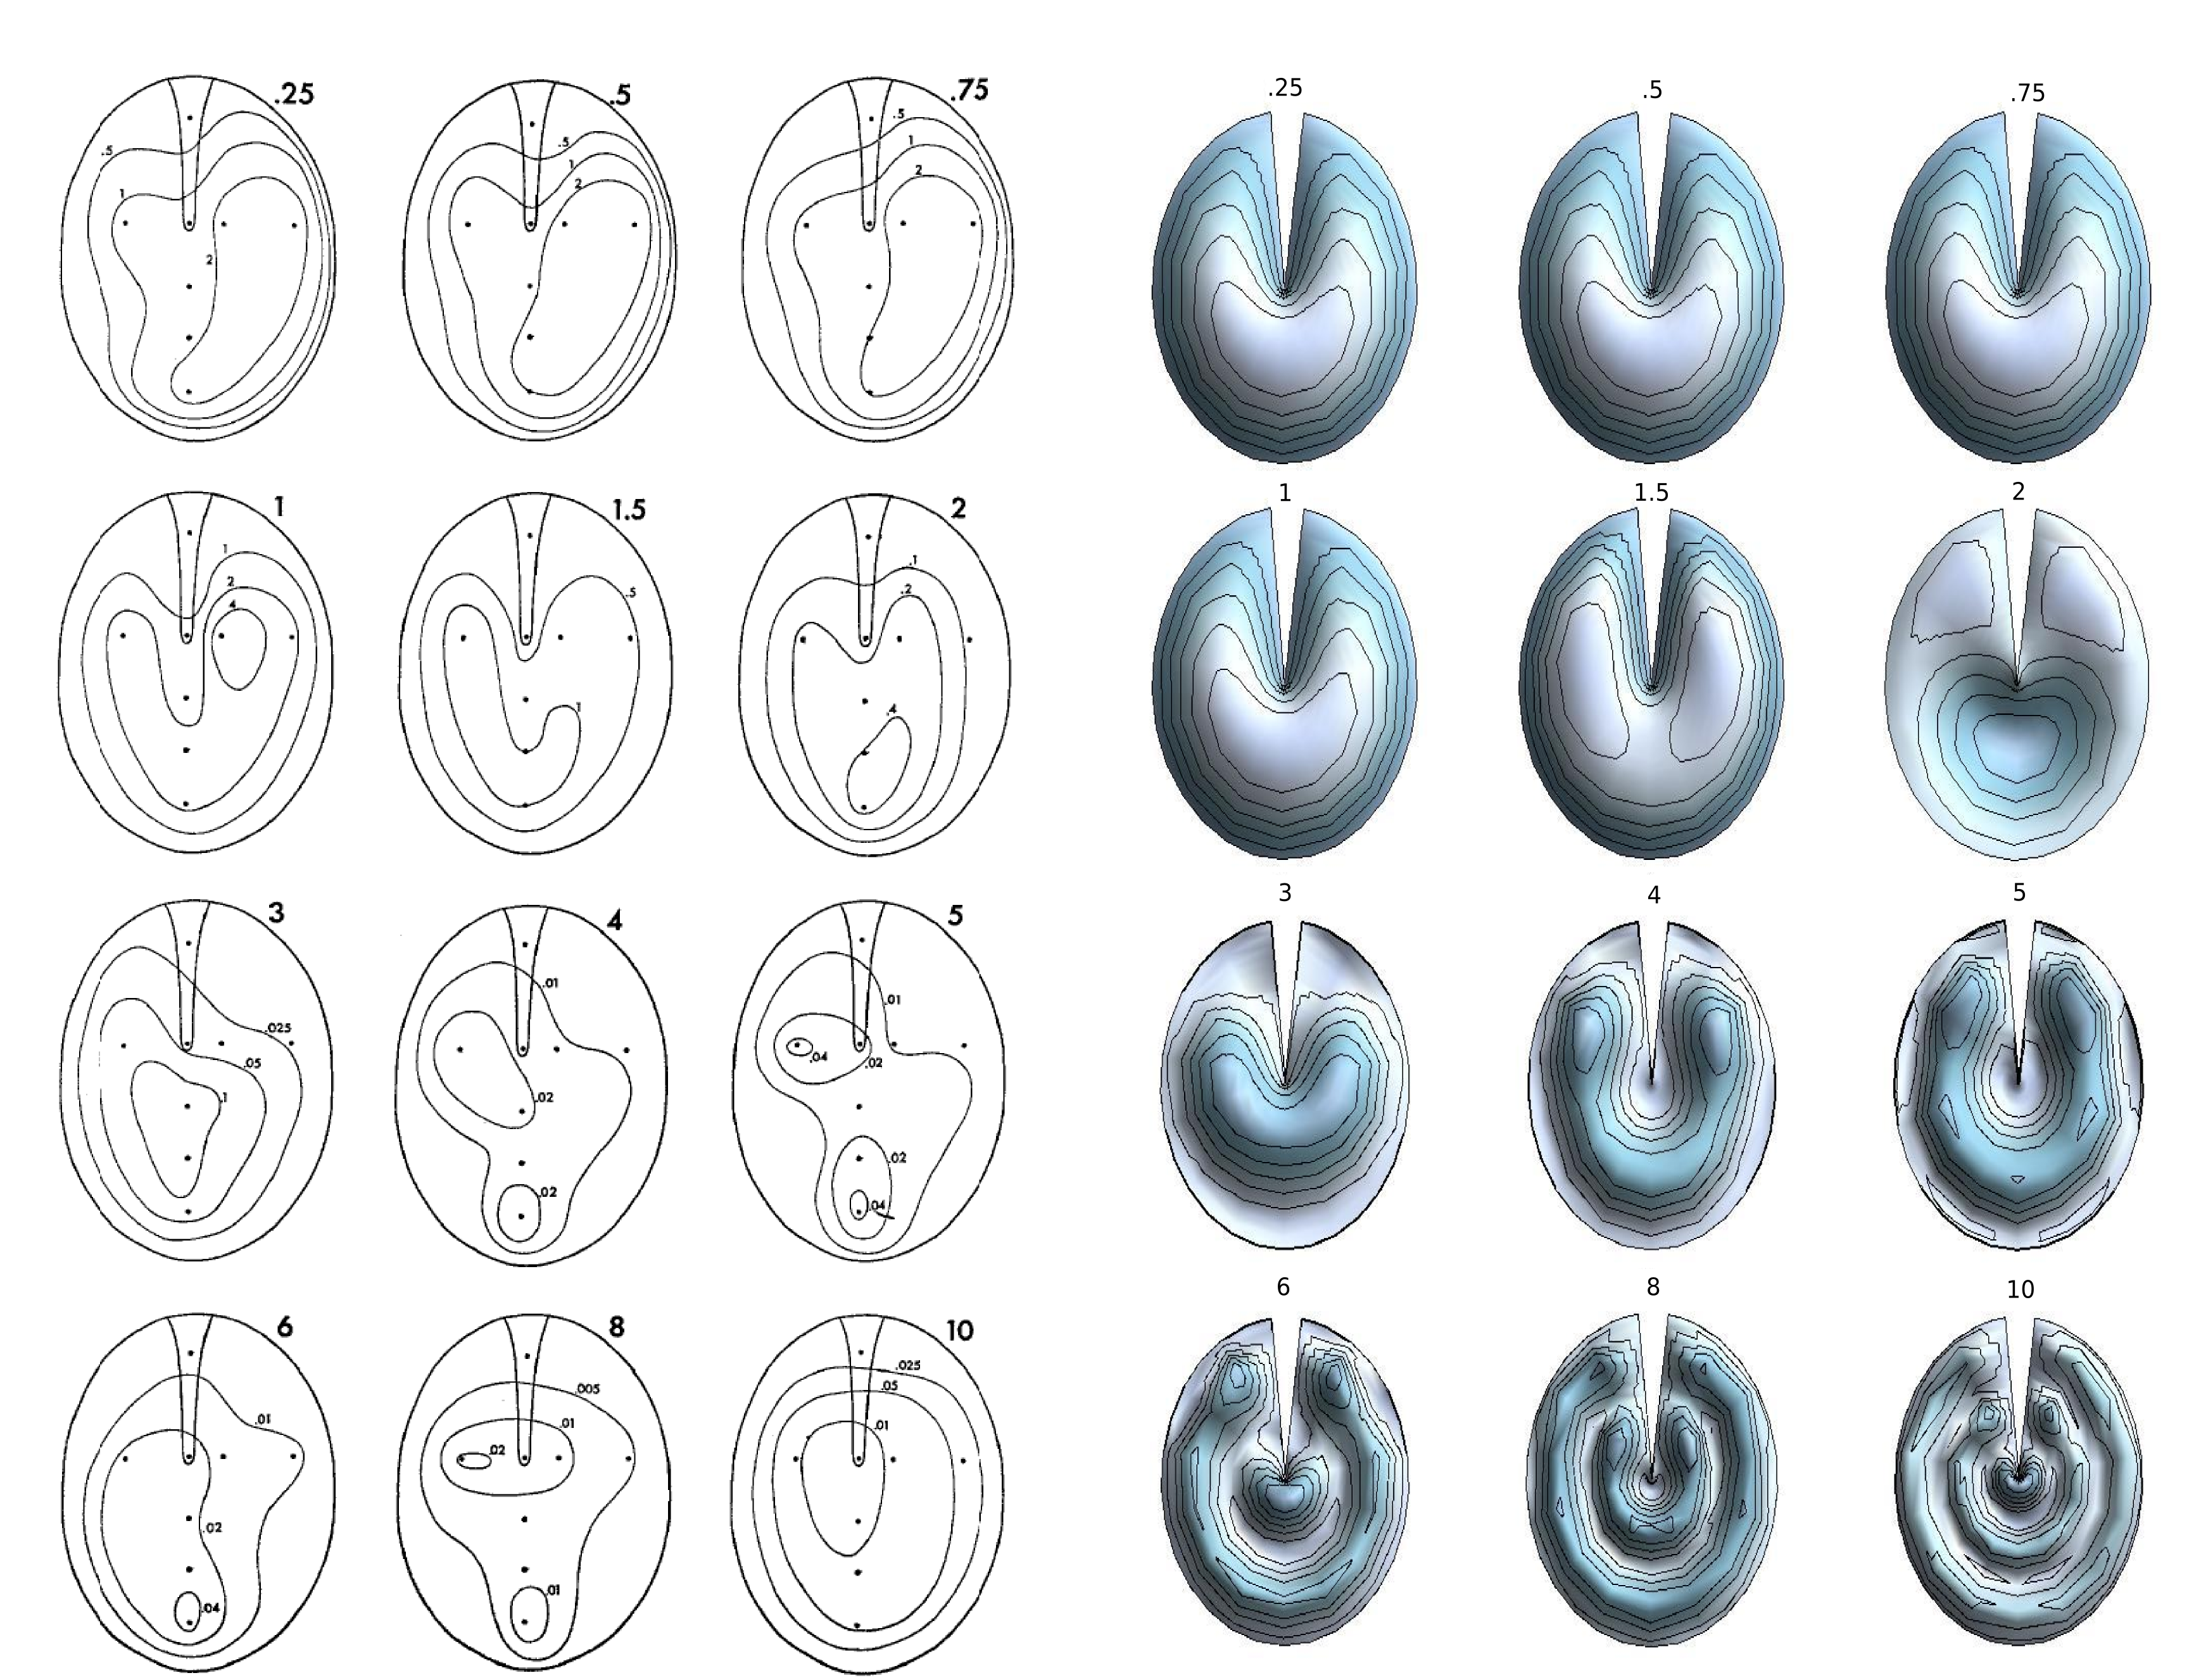
\includegraphics[width=1.0\linewidth]{Diagrams/manleymodelcomparison.png}
 \caption[Tokay gecko tympanum vibration profiles.]{Experimental membrane vibration patterns of the Tokay gecko dependent
 on sound frequency varying from $.5$kHz to $10$kHz. Data taken from \cite{manleygecko1}.}
  \label{manleygeckotympanum}
\end{figure}

In order to compare our model with the experimental results, we plot the response of one of the membranes ($x=0$, although $x=L$ could be
chosen equivalently due to the symmetry of the system) in our cylindrical ICE model 
calculated using \eqref{ipsimembranefull}. The opposite ear was chosen to be blocked, meaning $p_L=0$. 
This is illustrated in Fig. \ref{manleygeckotympanum} (right) for the same frequency range as in the experimental data. The sound pressure input was chosen to have unit amplitude and the model parameters used are given
on the right most column of Table \ref{geckogeometricparams}. The omitted region corresponds to the extracolumella. 

The asymmetric nature of our membrane vibration pattern is a result of our chosen geometry.
Mathematically this is a result of the fact that a uniform pressure (on the membrane surface) on a full circular membrane only couples to the circularly symmetric $J_0$ modes.
In the case of the sectoral membrane however, the uniform pressure couples to all the eigenmodes resulting in a more complex pattern.
As a qualitative reproduction our model is very accurate but for a full quantitative analysis, we would 
need to account for the motion of the extracolumella. Moreover, the full mechanics of the extracolumella including 
 its flection at higher frequencies can have significant effects which have not been studied so far.
% \begin{figure}[ht!]
%  \centering
%  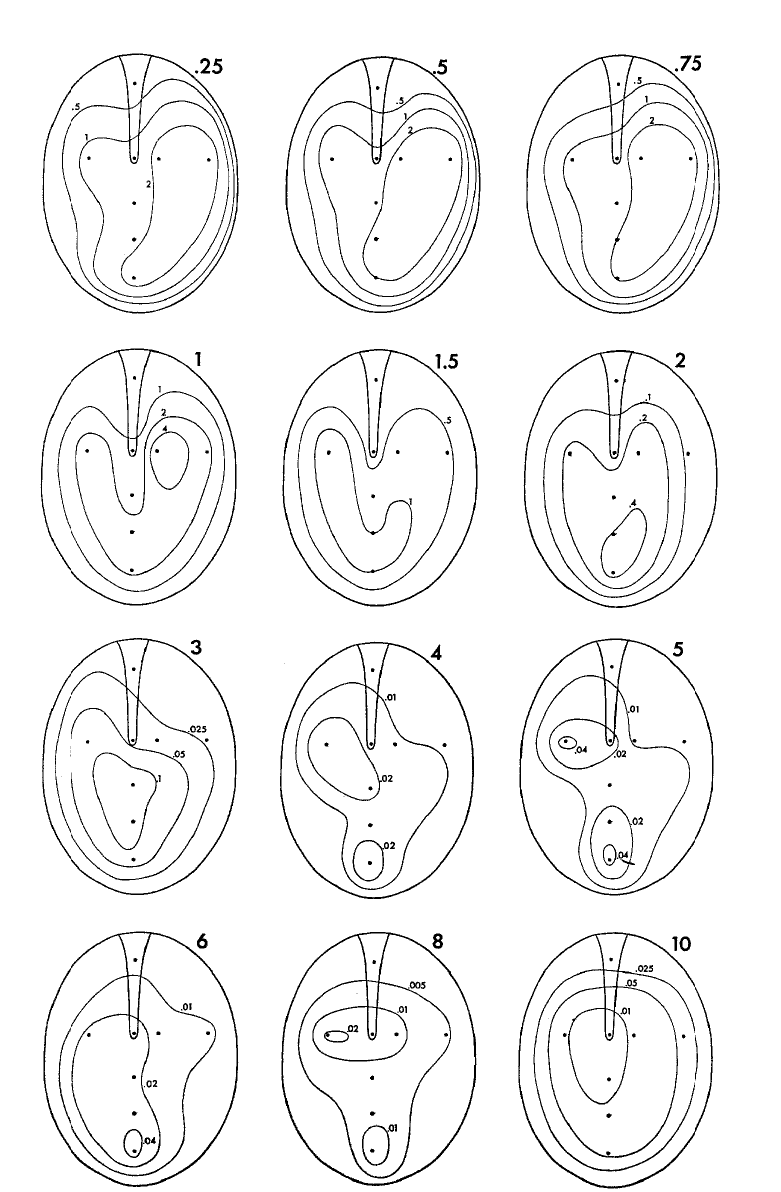
\includegraphics[width=.5\linewidth]{Diagrams/manleygeckoear2.png}
%  \caption[Tokay gecko tympanum vibration profiles.]{Experimental membrane vibration patterns of the Tokay gecko dependent
%  on sound frequency varying from $.5$kHz to $10$kHz. Data taken from \cite{manleygecko1}.}
%   \label{manleygeckotympanum}
% \end{figure}

% \begin{figure}[ht!]
%  \centering
%  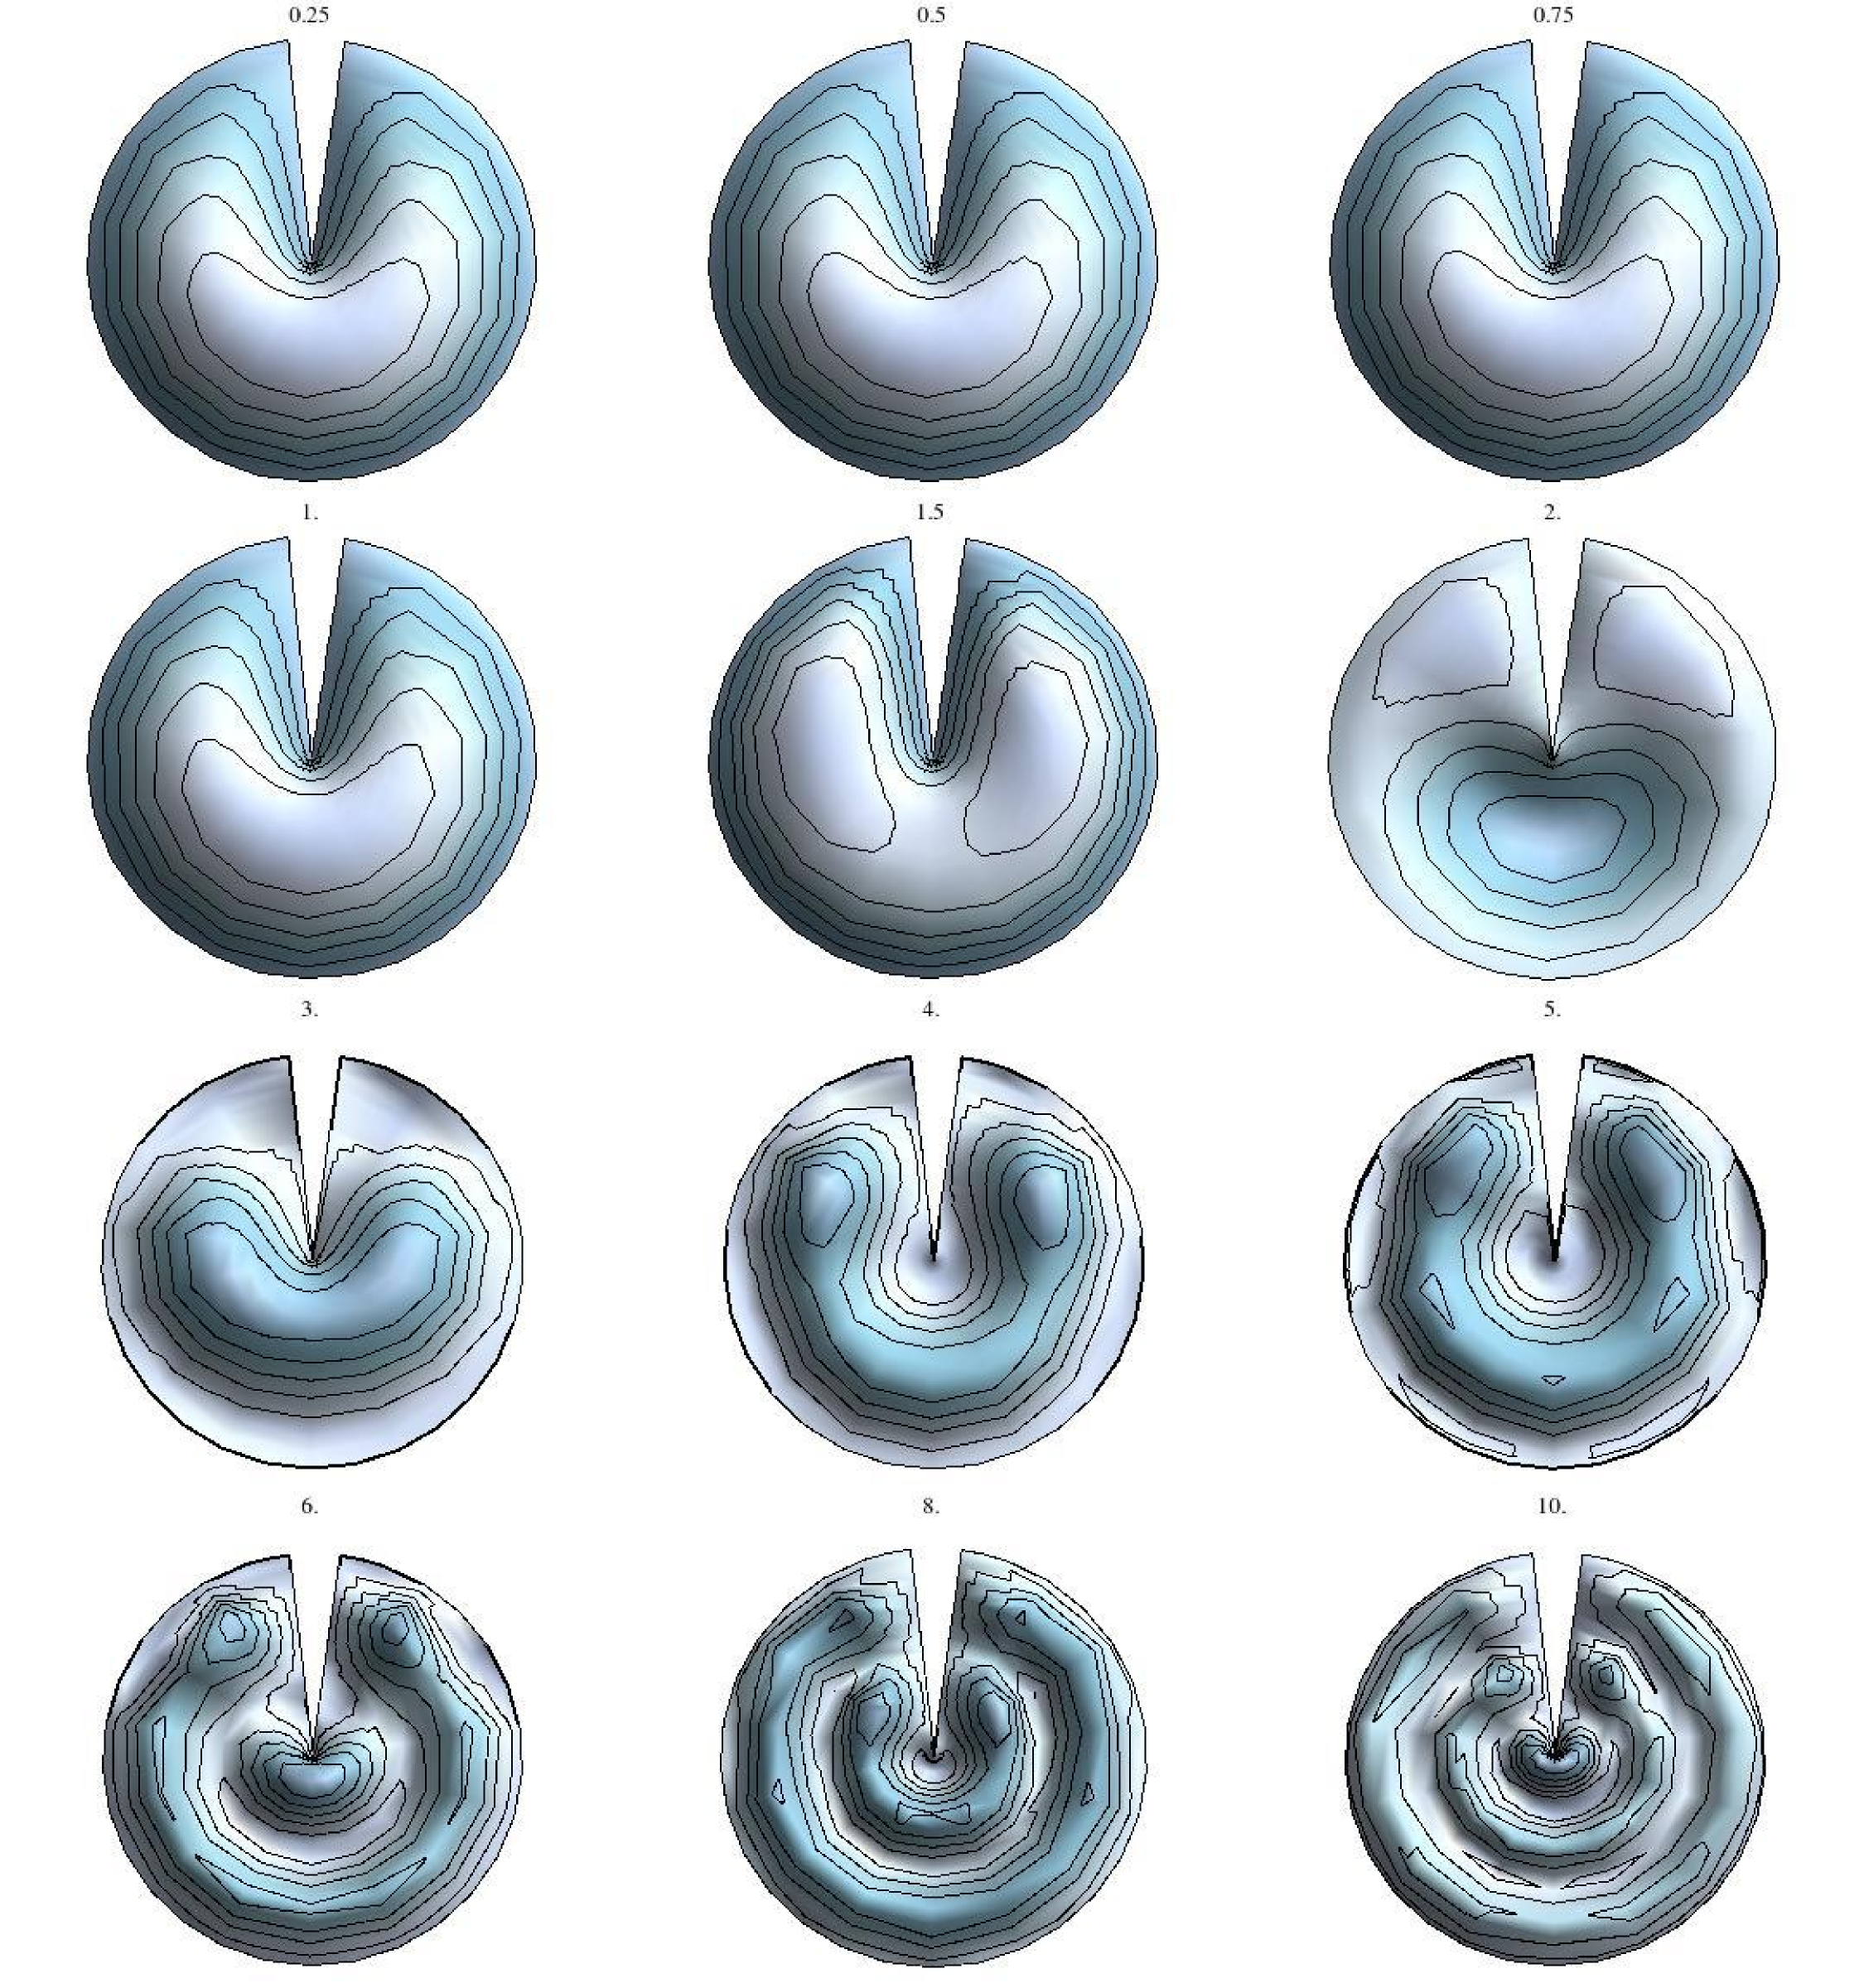
\includegraphics[width=.75\linewidth]{Diagrams/SectorMembraneModes/sector_membrane_all.png}
%  \caption[Sectoral membrane vibration profiles.]{Vibration patterns of a sectoral membrane
%  of radius $2.2$mm on sound frequency varying from $.5$kHz to $10$kHz. Compare with fig. \ref{manleygeckotympanum}}
%   \label{sectormembraneprofile}
% \end{figure}